% Drawing 154/05-7 -- folder 154, batch 05, archive page 97 (PDF page 98).
% Transcription: croquis en couleur sans phrase, sur une feuille de listing d'ordinateur (bandeau imprimé du 16 août 1982) : à droite, un disque traversé de pseudo-droites orange, deux petits arcs du bord renforcés en noir aux extrémités d'une corde, et un long arc noir en bas ; au milieu en bas, une bande (bords vert clair et noir, pleins ou en tirets, hachurée par endroits) coupée de droites orange, dont les bords se croisent en un point ; à droite en bas, un grand disque où un faisceau de pseudo-droites orange se tresse vers le haut, avec deux arcs du bord et un arc du bas renforcés en noir et des segments de bord marqués « $\frac12$ » ; enfin deux petits disques du même type, dans le second les segments de bord marqués « $\frac12$ », « $0$ », « $\frac12$ »
% Kind: disks with black boundary arcs; a band cut by orange lines. Method 2 (schematic redraw from the facsimile). Status: partial.
% Notes: On a printed listing sheet (CRAY2 job banner, 16 Aug 82; not reproduced). Right: a disk crossed by orange pseudolines, two short arcs of the rim reinforced in black at the ends of a chord, and a long black arc at the bottom. Middle bottom: a band (light green and black borders, solid or dashed, hatched in places) cut by orange lines, whose borders cross at a point. Bottom right: a large disk where a pencil of orange pseudolines braids upwards, two arcs of the rim and an arc of the bottom reinforced in black, stretches of rim marked « 1/2 »; and two small disks of the same type, in the second the stretches marked « 1/2 », « 0 », « 1/2 ». Read from the page view; strands schematic, hatching left out.
% Coordinates: 1 unit = 1 mm = 1/100 of the crop width (bbox in page fractions: [0.279, 0.185, 0.9, 0.528]).
% Redrawn by Claude (claude-opus-5-5), issue #73, 2026-11-07; not checked by a human; not compiled (no TeX in the session).
% Rights: reproduces part of the work -- behind RENDER_TRANSCRIPTS, never published by itself.
\documentclass[tikz,border=3pt]{standalone}
\usepackage{amsmath,amssymb}
\usetikzlibrary{patterns,arrows.meta}
\tikzset{Or/.style={orange!90!black}, Ye/.style={yellow!80!orange}, Lg/.style={green!60!black!70}, Dg/.style={green!45!black}, Br/.style={brown!80!black}, Rd/.style={red!85!black}, Bl/.style={blue!70!black}, Gy/.style={black!40}, pencil/.style={black!45}, struck/.style={black!35}, mark/.style={circle,draw,inner sep=1.3pt}, pt/.style={circle,fill,inner sep=0.9pt}, opt/.style={circle,draw,fill=white,inner sep=1.1pt}}
\begin{document}
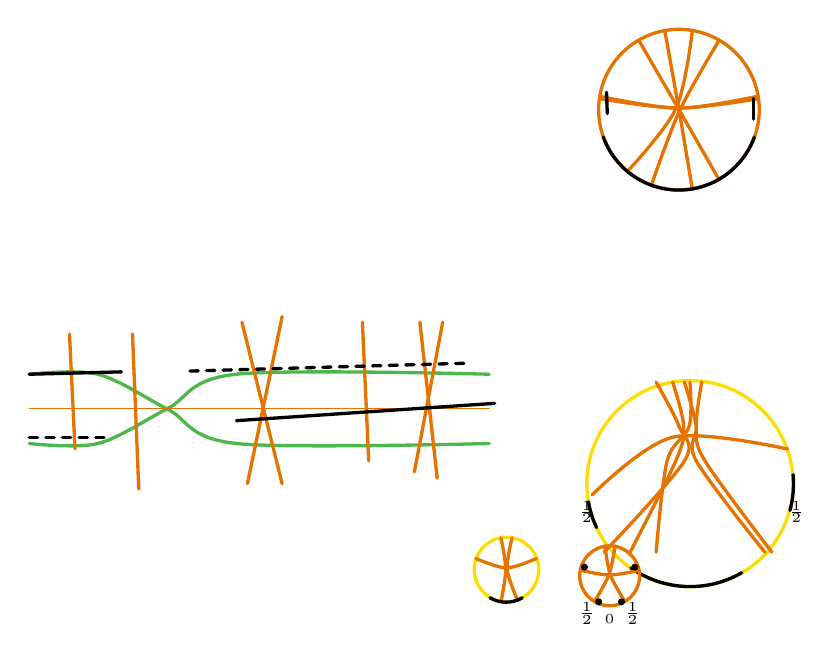
\begin{tikzpicture}[x=1mm,y=1mm,line cap=round,line join=round,font=\scriptsize]
\draw[Or,very thick] (84.7,-13.1) circle[radius=10.2];
\draw[Or,very thick] plot[smooth, tension=0.55] coordinates {(74.6,-11.4) (84.7,-12.9) (94.7,-11.4)};
\draw[Or,very thick] plot[smooth, tension=0.55] coordinates {(74.6,-11.7) (84.7,-12.9) (94.8,-11.7)};
\draw[Or,very thick] plot[smooth, tension=0.55] coordinates {(82.9,-3.1) (84.7,-13.1) (86.4,-23.2)};
\draw[Or,very thick] plot[smooth, tension=0.55] coordinates {(89.8,-4.3) (84.8,-13.2) (81.2,-22.7)};
\draw[Or,very thick] plot[smooth, tension=0.55] coordinates {(79.6,-4.3) (84.7,-13.1) (89.8,-22)};
\draw[Or,very thick] plot[smooth, tension=0.55] coordinates {(86.4,-3.1) (84.3,-13) (78.1,-21)};
\draw[very thick] (75.5,-10.9) -- (75.6,-13.6);
\draw[very thick] (94.2,-11.7) -- (94.2,-14.3);
\draw[very thick] (75.1,-16.6) arc[start angle=200, end angle=340, x radius=10.2, y radius=10.2];
\draw[Lg,very thick] plot[smooth, tension=0.55] coordinates {(2.2,-46.7) (10.9,-46.7) (19.7,-51.1) (28.5,-55.5) (60.6,-55.5)};
\draw[Lg,very thick] plot[smooth, tension=0.55] coordinates {(2.2,-55.5) (10.9,-55.5) (19.7,-51.1) (28.5,-46.7) (60.6,-46.7)};
\draw[Or] (2.2,-51.1) -- (60.6,-51.1);
\draw[Or,very thick] (7.3,-41.6) -- (8,-56.2);
\draw[Or,very thick] (15.3,-41.6) -- (16.1,-61.3);
\draw[Or,very thick] (29.2,-40.1) -- (34.3,-60.6);
\draw[Or,very thick] (34.3,-39.4) -- (29.9,-60.6);
\draw[Or,very thick] (44.5,-40.1) -- (45.3,-57.7);
\draw[Or,very thick] (51.8,-40.1) -- (54,-59.9);
\draw[Or,very thick] (54.7,-40.1) -- (51.1,-59.1);
\draw[very thick,dashed] (2.2,-54.7) -- (12.4,-54.7);
\draw[very thick,dashed] (22.6,-46.3) -- (57.7,-45.3);
\draw[very thick] (28.5,-52.6) -- (61.3,-50.4);
\draw[very thick] (2.2,-46.7) -- (13.9,-46.4);
\draw[Ye,very thick] (86.1,-60.6) ellipse[x radius=13.1, y radius=13.1];
\draw[Or,very thick] plot[smooth, tension=0.55] coordinates {(81.8,-47.7) (84.7,-53.3) (85.4,-57.7) (75.2,-69.3)};
\draw[Or,very thick] plot[smooth, tension=0.55] coordinates {(83.9,-47.7) (85.3,-53.3) (84.3,-57.7) (78.5,-69.3)};
\draw[Or,very thick] plot[smooth, tension=0.55] coordinates {(86.1,-47.7) (86,-53.3) (83.2,-57.7) (81.8,-69.3)};
\draw[Or,very thick] plot[smooth, tension=0.55] coordinates {(85.4,-47.7) (86.9,-53.3) (86.9,-57.7) (95.6,-69.3)};
\draw[Or,very thick] plot[smooth, tension=0.55] coordinates {(87.6,-47.7) (86.9,-53.3) (88,-57.7) (96.5,-69.3)};
\draw[Or,very thick] plot[smooth, tension=0.55] coordinates {(73.7,-62) (83.9,-54.7) (98.5,-56.2)};
\draw[very thick] (73.2,-62.9) arc[start angle=190, end angle=205, x radius=13.1, y radius=13.1];
\draw[very thick] (98.8,-64) arc[start angle=-15, end angle=5, x radius=13.1, y radius=13.1];
\draw[very thick] (78.6,-71.3) arc[start angle=235, end angle=300, x radius=13.1, y radius=13.1];
\node[inner sep=1pt] at (73,-64.2) {\tiny $\frac12$};
\node[inner sep=1pt] at (99.6,-64.2) {\tiny $\frac12$};
\draw[Ye,very thick] (62.8,-71.5) circle[radius=4.1];
\draw[Or,very thick] plot[smooth, tension=0.55] coordinates {(62.1,-67.5) (62.7,-71.5) (62.1,-75.6)};
\draw[Or,very thick] plot[smooth, tension=0.55] coordinates {(63.5,-67.5) (62.9,-71.5) (64.2,-75.4)};
\draw[Or,very thick] plot[smooth, tension=0.55] coordinates {(58.9,-70.1) (62.8,-71.3) (66.6,-70.1)};
\draw[very thick] (60.7,-75.1) arc[start angle=240, end angle=300, x radius=4.1, y radius=4.1];
\draw[Or,very thick] (75.9,-72.3) circle[radius=3.8];
\draw[Or,very thick] plot[smooth, tension=0.55] coordinates {(75.3,-68.5) (76,-72.2) (77.8,-75.5)};
\draw[Or,very thick] plot[smooth, tension=0.55] coordinates {(76.6,-68.5) (75.8,-72.2) (74,-75.5)};
\draw[Or,very thick] plot[smooth, tension=0.55] coordinates {(72.2,-71.6) (75.9,-72.2) (79.7,-71.6)};
\node[pt] at (72.7,-71.2) {};
\node[pt] at (79.1,-71.2) {};
\node[pt] at (74.5,-75.6) {};
\node[pt] at (77.4,-75.6) {};
\node[inner sep=1pt] at (73,-77.1) {\tiny $\frac12$};
\node[inner sep=1pt] at (75.9,-77.8) {\tiny $0$};
\node[inner sep=1pt] at (78.8,-77.1) {\tiny $\frac12$};
\end{tikzpicture}
\end{document}
